\chapter{Testování}
\label{sec:te}

%tady napsat nakej strucnej uvod jako je v tech predchozich kapitolach az budem mit tu propustnost

\section{Automatizované testy}

K~aplikaci jsem vytvořil sadu automatizovaných testů, které ověřují funkčnost jednotlivých komponent. Konkrétně jde o~testy pro \textit{model} aplikace (zde je testována především třída \texttt{Garage}), webové rozhraní a API systému. Tyto testy byly implementovány pomocí frameworku pytest \cite{pytest}.

Části aplikace, u~kterých je automatizované testování problematikcé, jako například funkce využívající APScheduler (viz sekci \ref{sec:im_scheduler}) nebo zasílání notifikací, jsem otestoval ručně.

\subsection{Testovací konfigurace}

Před spuštěním automatizovaných testů je nutné upravit konfiguraci aplikace. Především je třeba určit umístění testovací databáze a souboru s~uživatelským nastavením. Tyto soubory jsou v~průběhu testů upravovány a po dokončení smazány.

Také je nutné vypnout ochranu proti CSRF v~celé aplikaci, což výrazně zjednodušší testování formulářů aplikace. Jelikož požadavky s~metodou \texttt{post} vytvořené v~testech nepocházejí z~webových stránek aplikace, nemohou dodat CSRF \textit{token}, který je součástí formuláře. 

Sdílení \textit{tokenu} mezi aplikací a testy by sice bylo možné implementovat, bylo by však zbytečně komplikované. Za vhodnější postup považuji vypnutí CSRF ochrany pro většinu testů a funkčnost ochrany otestovat v~samostatném testu (viz sekci \ref{sec:te_csrf}).

Změna konfigurace aplikace je provadena nastavením proměnné prostředí \texttt{GARAGE\_SYSTEM\_CONFIG} na soubor s~testovací konfigurací (viz sekci \ref{sec:im_config}).

\subsection{Testování \textit{modelu}}
\label{sec:te_model}

Testování \textit{modelu} aplikace spočívá především v~testování metod třídy \texttt{Garage}. Třída \texttt{Event} slouží pouze k~uchování dat o~události a neimplementuje žádné metody, které by bylo možné testovat.

Testovány jsou následující scénáře:

\begin{itemize}
    \item Přidání garáže.
    \item Smazání garáže.
    \item Kontrola zmeškaných hlášení.
    \item Zaslání kontrolního hlášení.
    \item Změna stavu po zaslání události.
    \item Zneplatnění API klíče.
    \item Získání zaznamenaých událostí podle typu.
\end{itemize}

Zde stojí za zmínku test kontroly zmeškaných hlášení. V~něm je garáži zasláno kontrolní hlášení, čímž je určen čas dalšího očekávaného hlášení. Po překročení tohoto času je potřeba otestovat, zda byl stav garáže změnen na \uv{Nehlásí se}.

Jelikož je minimální perioda hlášení 1 minuta, prosté čekání (například pomocí funkce \texttt{sleep()}) by proces testování neúnosně zpomalilo (pro srovnání spuštění všech testů aplikace na běžném počítači zabere asi 4 sekundy). Vhodnější je tedy časový posun nasimulovat.

K~tomu je použita knihovnu FreezeGun \cite{freezegun}. Tato knihovna umožňuje explicitně nastavit datum a čas, které vrátí funkce \texttt{now()}, používaná v~implementaci třídy \texttt{Garage}. Použití knihovny při testování kontroly promeškaných hlášení je demonstrováno v~ukázce \ref{lst:freezegun}.

\begin{listing}[htbp]
\caption{\label{lst:freezegun} Test kontroly promeškaných hlášení. Pomocí knihovny FreezeGun je čas nastaven na půlnoc 1. 1. 2011. Poté je čas posunut o~dvě hodiny a otestována změna stavu garáže.}
\inputminted[bgcolor=codebg]{python}{source-samples/freezegun.py}
\end{listing}

\subsection{Testování API}

Testy API nadřazeného systému ověřují funkčnost následujících operací:

\begin{itemize}
    \item Vytvoření garáže při vypnutném registračním módu.
    \item Zaslání události.
    \item Zaslání události s~neplatným API klíčem.
\end{itemize}

U~každého testu je zkontrolováno, zda byla odeslána správná odpověď na příslušný požadavek -- návratový kód (například \textit{404 -- Forbidden}) a zaslaná data. Je tedy testována pouze reakce API \textit{controlleru}, vliv operací na databázi nadřazeného systému je pokryt v~testu \textit{modelu} (viz sekci \ref{sec:te_model}).

\subsection{Testování webového rozhraní}

V~těchto testech je zkoumán \textit{controller} webového rozhraní a zobrazované HTML stránky. Testovány jsou tyto scénáře:

\begin{itemize}
    \item Zobrazení hlavní stránky.
    \item Zobrazení stránky garáže.
    \item Zobrazení událostí.
    \item Zobrazení chybové stránky při zadání neexistující garáže.
    \item Filtrování událostí.
    \item Úprava dat garáže (označení, poznámka a telefonní číslo), včetně testu ověření neplatných hodnot.
    \item Úprava uživatelského nastavení (telefonní číslo pro zasílání upozornění).
\end{itemize}

V~každém testu je ověřováno, zda aplikace v~reakci na požadavek vygeneruje odpovídající webovou stránku a vrátí odpovídající návratový kód.

Zobrazení testovaných stránek vyžaduje přihlášení do webového rozhraní nadřazeného systému. To by vyžadovalo zaslání přihlašovacího požadavku se správným heslem před spuštěním testů.

Další možnost je nastavit přihlášení explicitně, modifikací testovací HTTP relace. Proto není nutné spoléhat na funkcionalitu přihlašování, která je testována samostatně.

Framework Flask umožňuje k~aplikaci vygenerovat testovacího klienta, jehož relaci je možné libovolně modifikovat \cite{flask_testing}. Díky tomu lze nastavit proměnnou \texttt{logged\_in}, která je používána ke kontrole přihlášení (viz sekci \ref{sec:im_auth}). Nastavení této proměnné je provedeno způsobem naznačeným v~ukázce \ref{lst:logged_in}.

\begin{listing}[htbp]
\caption{\label{lst:logged_in} Explicitní nastavení proměnné \texttt{logged\_in} na požadovanou hodnotu. Pomocí takto modifikovaného testovacího klienta lze zasílat požadavky, na které bude aplikace reagovat jako při přihlášení.}
\inputminted[bgcolor=codebg]{python}{source-samples/logged_in.py}
\end{listing}

\subsection{Testování autentizace uživatele}

Toto testování ověřuje jednak funkci \textit{controlleru} provádějícího autentizaci, jednak přístup k~souboru s~uloženým otiskem hesla. Jsou zde testovány tyto scénáře:

\begin{itemize}
    \item Zobrazení přihlašovací stránky.
    \item Kontrola přihlášení při přístupu k~dalším částem systému (viz sekci \ref{sec:im_auth}).
    \item Přihlášení pomocí implicitního hesla.
    \item Zadání neplatného hesla.
    \item Odhlášení.
    \item Změna hesla.
\end{itemize}

Opět jsou kontrolovány návratové kódy odpovědí. Také je testováno, zda byla provedena příslušná přesměrování (například přesměrování na přihlašovací stránku při pokusu o~přístup k~částem rozhraní bez přihlášení) a zobrazení chybových hlášek (například při zadání neplatného hesla).

\subsection{Testování ochrany proti CSRF}
\label{sec:te_csrf}

Jelikož byla u~předchozích testů vypnuta ochrana proti CSRF, je vhodné provést ještě jednoduchý test, který ověří její fungování. Zde stačí zaslat testovanému formuláři data pomocí metody \texttt{post} bez platného CSRF \textit{tokenu}.

Výchozí chování CSRF ochrany ve frameworku Flask je v~případě chybějícího nebo neplatného \textit{tokenu} zaslat návratový kód \textit{400 -- Bad request} \cite{flask_wtf}. V~těle odpovědi je pak informace o~problému s~\textit{tokenem}. Stačí tedy otestovat návratový kód a obsah odpovědi (viz ukázku \ref{lst:csrf_test}).

\begin{listing}[htbp]
\caption{\label{lst:csrf_test} Test ochrany proti CSRF.}
\inputminted[bgcolor=codebg]{python}{source-samples/csrf_test.py}
\end{listing}

\section{Testovací nasazení aplikace}
\label{sec:te_deployment}

V~rámci testování jsem se rozhodl nasadit aplikaci nadřazeného systému na virtuálním serveru, způsobem popsaným v~sekci \ref{sec:an_cloud}. Tím je jednak otestován průběh nasazování aplikace, jednak je běžící aplikaci možné použít pro demonstrační účely. Aplikace je momentálně\footnote{Aplikace byla spuštěna 30. 3. 2018. Jelikož je registrace domény platná do 30. 6. 2018, bude její provoz po tomto datu ukončen.} přístupná na doméně \url{https://demo-garaze.tk}.

Jelikož je aplikace dostupná z~internetu, není vhodné použít k~provozu HTTPS \textit{self-signed} certifikát. Místo toho je k~doméně registrován platný certifikát autority Let's Encrypt.

Aplikace k~provozu využívá server Apache2. Při konfiguraci HTTPS na tomto serveru jsem vycházel z~článku \textit{Strong SSL Security on Apache2} \cite{apache_ssl}. Správnost konfigurace a platnost certifikátu byla ověřena pomocí testu poskytovaného společností Qualys. Výsledné hodnocení je možné vidět na obrázku \ref{fig:ssl_test}.

\begin{figure}[h!]
    \centering
    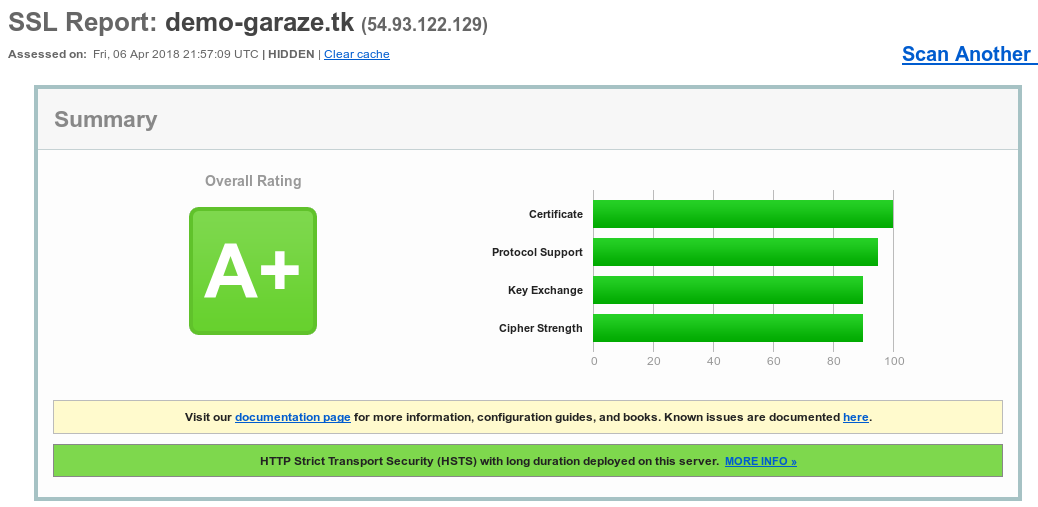
\includegraphics[width=\textwidth]{images/ssl_test.png}
    \caption[Výsledky testu HTTPS konfigurace]{Výsledky testu HTTPS konfigurace poskytnutného společností Qualys.}
    \label{fig:ssl_test}
\end{figure}

% napsat ze sme pri nasazovani prisli na novy chyby, ktery nebyly na lokale videt -- to s tim vodhlasovanim a secret_key, a to ze apache zahazuje ty headery s nepovolenejma znakama
Nasazení aplikace v~reálném prostředí odhalilo několik chyb, které nebyly při lokálním testování patrné. V~první řadě se ukázalo, že server Apache2 od verze 2.4 ignoruje v~příchozím požadavku hlavičky, které obsahují podtržítka \cite{apache_headers_update}. Podtržítka byla původně použita při zasílání hlavičky s~API klíčem (původně \texttt{api\_key}). Tuto chybu jsem opravil přejmenováním hlavičky na \texttt{apikey}.

Druhá chyba se týkala nastavení hodnoty \texttt{secret\_key} v~konfiguračním souboru aplikace. Tento klíč slouží k~podepisování HTTP relace či generování CSRF \textit{tokenů} \cite{flask_api}. V~konfiguraci aplikace použité při lokálním testování byl klíč vždy nastaven na náhodně vygenerovanou hodnotu.

Po nasazení se ukázalo, že WSGI \cite{python_wsgi} modul použitý pro spárování Python aplikace se serverem Apache2 tuto aplikaci v~některých případech restartuje. To by obecně ničemu nevadilo, nicméně při každém restartu byla znovu vygenerována nová hodnota \texttt{secret\_key}, což vedlo k~zneplatnění všech aktivních HTTP relací a CSRF \textit{tokenů}. Uživatel rozhraní tak byl náhle odhlášen nebo nemohl odesílat formuláře. 

V~konfiguračním souboru aplikace, který je použit při jejím nasazení, bylo proto generování klíče nahrazeno pevnou hodnotou (dostatečně dlouhým náhodně generovaným klíčem, který však není reinicializován při restartu aplikace).

% tady by se este dalo napsat ze sme meli preklep v tim apache konfiguraku a proto to wsgi nebezelo v tim daemon modu, a proto byly ty restarty vod nej tak casty, viz https://stackoverflow.com/questions/48507267/mod-wsgi-keeps-restarting-flask-app#comment84021510_48507792

% nicmene to ze generovat ten klic pokazdy je taky spatnej napad je taky pravda viz https://stackoverflow.com/questions/27287391/why-not-generate-the-secret-key-every-time-flask-starts

\subsection{Provozní server}

Aplikace byla nasazena na virtuálním serveru ze služby Amazon EC2, s~jedním procesorovým jádrem a 1 GB paměti. Použit byl operační systém Ubuntu Xenial 16.04.

\section{Simulátor podřízeného systému}

V~rámci testování aplikace nadřazeného systému jsem vytvořil simulátor podřízeného systému. Ten umožňuje snadné zasílání požadavku na API nadřazeného systému, podobně jako by to dělal reálný podřízený systém.

Simulátor je implementován jako jednoduchá stránka, která je součástí webového rozhraní nadřazeného systému. Zasílání požadavků je realizováno pomocí Javascriptu a knihovny jQuery \cite{jquery_about}. 

Stránka simulátoru je přístupná na \texttt{/simulator}, pokud byla aplikace nadřazeného systému spuštěna v~ladícím módu (\texttt{DEBUG = True} v~konfiguračním souboru aplikace).

\section{Test odezvy nadřazeného systému}
\label{sec:te_lat}

V~závěru testování jsem vyzkoušel dobu odezvy nadřazeného systému při nasazení na Raspberry Pi 3. Chtěl jsem ověřit především dobu zpracování události zaslané podřízeným systémem.

Při testu se ukázalo, že doba odezvy roste s~počtem událostí, které byly pro danou garáž zaznamenány. Zpočátku byly zaslané události zpracovány zhruba za 150 až 200 milisekund. Pokud však měla daná garáž v~databázi uloženo již kolem 2000 událostí, vzrostla doba zpracování až na 800 milisekund.

Příčinou byl výchozí způsob, kterým framework SQLAlchemy mapuje databázové záznamy na Python objekty. Problém byl vyřešen dynamickým načítáním záznamů, které je popsáno v~sekci \ref{sec:im_lazy}. Po této úpravě se doba odezvy ustálila na přibližně 200 milisekudnách, bez ohledu na počet zaznamenaných událostí.

% napsat ze sme vodhalili ten problem s lazy loadingem viz http://docs.sqlalchemy.org/en/latest/orm/collections.html, napsat neco v tom smyslu, ze ten normalni loading co tam je je pomalej pro velky kolekce jako sou ty udalosti a ze se musi pouzit trochu jinej pristup. ruzny strategie sou popsany v tim clanku, a ze my sme zvolili to prvni, teda pouziti dynamic loadingu (muzu napsat ze sme este zkouseli noload).

% este napsat ze s tim dynamic loadingem nejde ke kolekci garage.events pristupovat primo, takze sme udelali funkci garage.get_events(event_type=None), ktera nam ten pristup zapouzdri a este s ni muzem filtrovat podle typu

% tzn ten tradeoff je ze ted to garage.events neni primo kolekce ale nakej query object kterej nevobsahuje vsechnny ty eventy, ale to nevadi protoze k tem eventum stejne pristupujem jen pres to get events. Este tam muzem napsat ze misto toho dynamickyho loadovani bysme mohli dat ten noload a nenacitat ty eventy vubec a pak v ty metode get_events misto toho query objectu co vraci to dynamicky loadovani (pres relationship) bysme pouzivali proste tu tridu Event, stylem Event.query... ale tohle ze je takovy cistsi.

% prave ten hlavni problem ty python kolekce je ze se do ni pri tim appendu musej nacist vsechny ty vobjekty, coz je zbytecny a drahy. Kdezto pri tim dynamickym loadu je to nenacita protoze jakoby ten append nepristupuje k python kolekci ale k nakymu tomu query objektu (vytvorenymu zas pres ten relationship).

% este napsat ze bez toho se pridavani udalosti ke garazim ktery jich uz maj moc furt spomalovalo kvuli tomu appendu, takhle je to +- stejny furt i pro mega udalosti.

% tohle vsechno vychazi z toho collections clanku

% nakonec napsat ze se to da este trochu zrychlit pouzitim tech sessions v requests
